\documentclass[12pt]{amsart}
\usepackage{amsmath}
\usepackage{tikz,float,caption}
\usetikzlibrary{arrows.meta,calc,decorations.markings,patterns,cd,patterns.meta}

\begin{document}

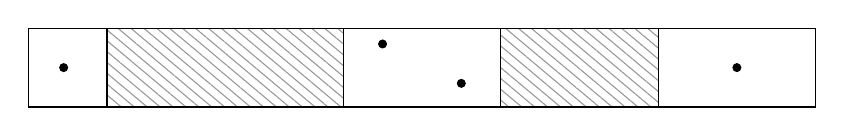
\begin{tikzpicture}
    \fill[pattern={Lines[angle=-40]},pattern color=black!40!white] (1,0) rectangle (4,1);
    \fill[pattern={Lines[angle=-40]},pattern color=black!40!white] (6,0) rectangle (8,1);
    \draw (0,0) rectangle (10,1);
    \foreach \x in {1,4,6,8} {
      \draw (\x,0)--+(0,1);
    }
    \path[every node/.style={draw,circle,inner sep=1pt,fill}] (0,0.5)--+(0.45,0)node{}--+(4.5,0.3)node{}--+(5.5,-0.2)node{}--+(9,0)node{};
  \end{tikzpicture}

\end{document}